%\section{Consolidation des Connaissances et rappel (09/01/2012)}

\abstractframe{En introduction au cours, une suite de rappels et de définitions sont effectués dans
ce chapitre. Cette démarche assure la mise en place d'une sémantique et d'une terminologie commune. En
outre, lors du parcours des rappels et des prérequis, une intention particulière est portée sur les
éléments qui seront essentiels de retenir pour les prochains chapitres.}
{../img/overview.png}

\section{Rappel} % (09/01/2012)}

\subsection{Processeur, entrées/sorties et réseaux}

\ifbook{

  \subsubsection{Fonctionnement schématique d'un ordinateur}

  \paragraph{} Avant d'entrer dans les coeur du sujet, il est nécessaire de tout d'abord bien
  comprendre comment fonctionner la brique la plus élémentaire de tout système informatique:
  l'ordinateur.

  \begin{figure}[hb]
    \begin{center}
      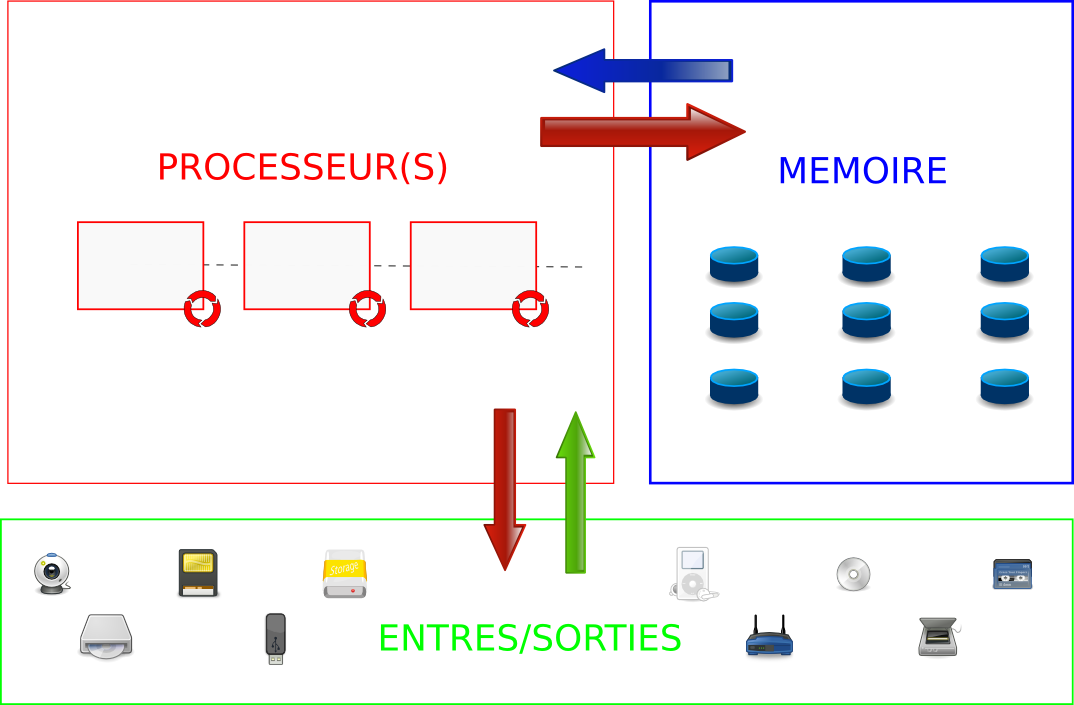
\includegraphics[scale=0.3]{img/cpu-schematics.png}
      \caption{Schéma simplifié du fonctionnement d'un ordinateur}
      \label{schema-ordi}
    \end{center}
  \end{figure}

  \paragraph{} Comme l'illustre le dessin (TODO), un ordinateur, aussi complexe soit-il peut être
  résumé aux trois composants suivants:
  \begin{description}
    \item[Processeur] unité de traitement de l'ordinateur, c'est lui qui réalise les calculs et qui
    produit les résultats.
    \item[Mémoire] espace de travail du processeur, la mémoire lui permet de placer les résultats,
    intermédiaires ou finaux, de ses calculs
    \item[Entrées/Sorties] pour communiquer avec le "monde extérieur" (clavier, écran, disques durs,
    réseaux,...) l'ordinateur disposent de différents composant matériels dédié aux différentes
    entrées/sorties avec qui il interagit.
  \end{description}

  \paragraph{Distinction mémoire vive et mémoire morte} Sans rentrer dans les détails techniques, il
  est important de noter que conceptuellement les périphériques de stockage, tel que les disques durs,
  ne sont pas conceptuellement très différent de la mémoire. Dans les deux cas, ils permettent au
  processeur de stocker des résultats.

  \paragraph{} Ce qui sépare donc ces deux composants est leur \textbf{persistence}. L'information
  située en mémoire est \textbf{volatile}, elle disparait si l'ordinateur s'éteint brusquement. À
  l'inverse, les données placées sur un périphérique de stockage, persiste au délà de l'extinction de
  l'ordinateur.
}

\ifslide{
  \begin{frame}{Qu'est-ce qu'un ordinateur ?}
   \begin{center}
     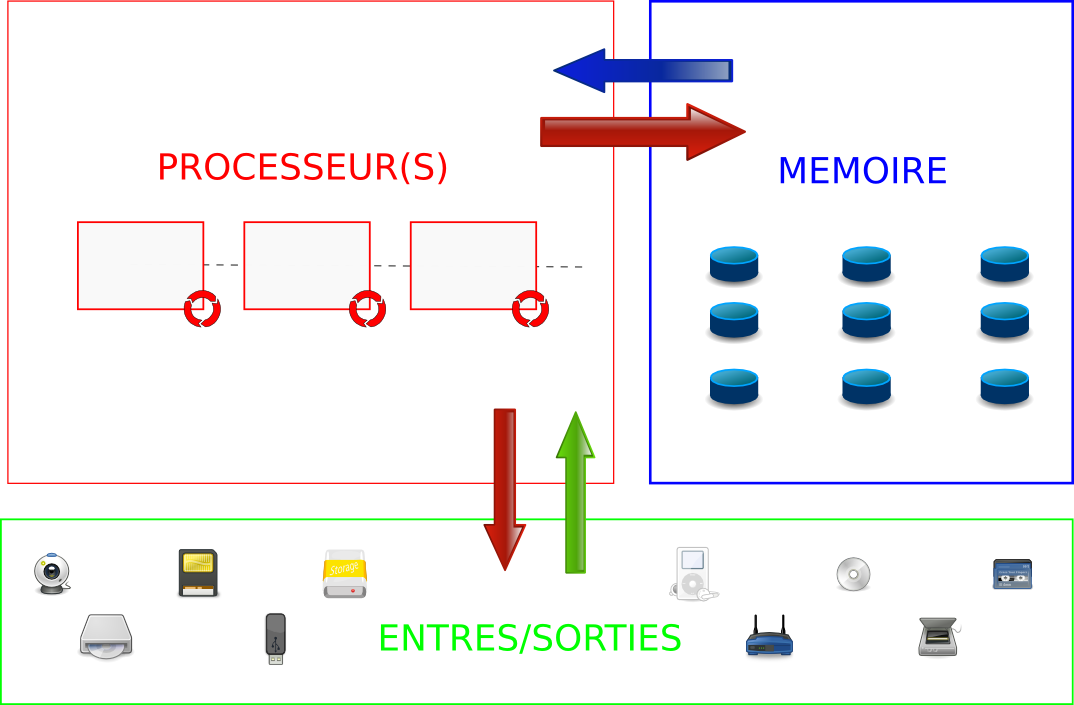
\includegraphics[scale=0.3]{img/cpu-schematics.png}
   \end{center}
  \end{frame}
}

\ifbook{
    \subsubsection{Rôle du système d'exploitation}

    \paragraph{} Encore une fois de manière très schématique, et surtout en restant pertinent par
    rapport au thème du cours, le \textit{Middleware}, nous allons maintenant brièvement évoqué le
    rôle du système d'exploitation.

    \paragraph{} En repartant de ce que nous venons de détailler sur le fonctionnement d'un
    ordinateur, plusieurs points peuvent rapidement être gênants. Le principal est que le processeur
    n'exécute qu'un seul programme à la fois, donc tel quel, seule une application peut s'exécuter
    sur un ordinateur.

    \paragraph{} Le système d'exploitation est une couche logicielle qui va permettre aux programmes
    s'exécutant sur l'ordinateur de se partager les resources mises à disposition par l'ordinateur
    (processeur, mémoire, périphériques de stockage,...). En outre, le système d'exploitation va
    jouer le rôle d'arbitre entre ses différents programmes, leur attribuant, chacun à leur tour, un
    certain temps d'utilisation de ces resources.

    \paragraph{} Ainsi, c'est grâce aux systèmes d'exploitation que de multiples programmes vont
    pouvoir s'exécuter en \textbf{parallèle} sur une machine, qu'elle possède un ou plusieurs
    processeurs.

    \paragraph{} Il est important de noter qu'aucun ordinateur ne pourra effectuer plus de tâches en
    parallèle que son nombre de processeurs, mais les cycles d'exécutions étant extrêmement rapide,
    un seul ordinateur, équippé d'un seul processeur, peut donner l'impression à son utilisateur
    d'exécuter simulatannéemnt plusieurs tâches. C'est l'impression que vous donne tous les jours,
    les ordinateurs dédiés à la bureautique que vous utilisez.

    \paragraph{Remarque} On notera aussi au passage qu'un même programme peut lui même se diviser en
    plusieurs processus distinct, s'exécutant aussi en parallèle, selon les règles évoqués juste
    avant. Ainsi, dans la cadre d'un projet \textit{middleware} la question de l'exécution, de
    manière concurrente, de différentes parties de l'application peut se poser... (Nous y
    reviendrons plus loin dans le cours).
}

\ifslide{
  \begin{frame}{Le rôle du système d'exploitation}

  \end{frame}

  \begin{frame}{Virtualisation \& "Cloud computing"}
  \end{frame}
}

\ifbook{
  \subsubsection{Limites physique d'un ordinateur}
  \paragraph{} Avant d'aller plus loin, arrêtons nous un instant sur ces notions et sur le système,
  aussi schématique soit-il que nous venons de décrire. Au regard de son fonctionnement, quelles
  limites pouvons nous déjà percevoir ? Dans quelle condition, une tel système - l'ordinateur, aura
  des difficultés à effectuer les opérations qu'on lui confie ?

  \paragraph{} Sans surprise, on peut distinctuer à peu près autant de limite que de composants
  distingué dans la précédente représentation. Etudions, sommairement, pour chacun d'entre eux les
  limites qu'ils induisent sur l'ordinateur.

  \paragraph{Processeur} La première limite physique d'un ordinateur, qui est pratiquement
  incontournable, est le processeur. Un processeur peut effectuer un certains nombres d'opérations
  dans un certain délai. Dans un système parfaitement optimisé, où tous les autres - assez
  nombreux, nous allons le voir, goulots d'étranglement ont été "neutralisés", cette vitesse
  d'exécution est une limite incompressible : l'ordinateur ne pourra simplement exécuter les
  opérations demandées plus rapidement...

  \paragraph{Parallélisme} Comme évoqué lors de la description du rôle d'un système d'exploitation,
  un ordinateur exécute souvent plusieurs processus à la fois, souvent plus nombreux que son nombre
  de processseur. Ainsi, il doit passer d'un processus à un autre, à tour de rôle, pour permettre à
  tous de s'exécuter \textit{presque} en parallèle.

  \paragraph{} Il évident le passage d'un processus à un autre  n'est pas gratuit, et nécessite, de
  la part du système d'exploitation, comme du processeur, un travail supplémentaire qui consiste à
  sauvegarder les données et l'état du processus placé en "pause" et à recharger ceux du processus
  qui "reprend la main".

  \paragraph{} Au bout du compte, si l'ordinateur effectue un nombre de tâches en parallèle
  largement trop grande pour sa capacité, il risque de passer plus de temps à \textbf{changer de
  contexte} entre chaque processus, pluôt qu'à réellement effecuter les opérations qu'on lui
  demande.

  \paragraph{Mémoire} La mémoire à la disposition du processeur impacte généralement grandement la
  vitesse d'exécution. En effet, plus l'ordinateur pourra placer de données en mémoire, plus il
  pourra avoir à sa disposition des résultats intérmédiaire et finaux.

  \paragraph{} Illustrons rapidement ce point par un exemple concret. Supposons que l'on confie à
  l'ordinateur de trier un tableau de données, composé d'une seule colonne, par ordre de grandeur
  croissante du contenu de chaque cellule:
}
%TODO: dessins
\ifslide{
  \begin{frame}{Exemple d'algorithme}
  \end{frame}
}
\ifbook{
  \paragraph{} Si l'ordinateur ne peut stocker qu'un seul résultat intermédiaire, en l'occurence la
  taille du contenu de la cellule, il ne peut réordonner le tableau que en échangeant les cellules
  de positons. En effet, il peut calculer la taille d'une cellule, la stocker, calculer la taille de
  la seconde cellule, la comparer à la précédente et changer l'ordre des deux cellules, si
  nécessaire, puis continuer...

  \paragraph{} Après un laborieux travail, cet \textbf{algorithme} sera capable de réordonner
  l'ensemble du tableau, mais en effectuant un important nombre de calculs. À l'inverse, si le
  processeur est libre de placer autant de résultats en mémoire que d'entrées dans le tableau, il
  pourra se contenter de calculer, une fois pour toute, la taille de chaque cellule, puis de les
  trier de manière plus "globale"...

  \paragraph{Remarque} Cet exemple est volontairement très grossier et n'est pas représentatif du
  tout du fonctionnement interne réel d'un ordinateur, ni même de la manière dont processeur va
  implémenter un algorithme de trie. Néanmoins, sans être l'exemple le plus respectieux des détails
  technique d'un ordinateur, il illustre de manière très juste l'importance de la mémoire pour la
  réalisation d'opération au sein d'un ordinateur.

  \paragraph{Entrées/Sorties} Après la mémoire, c'est très certainement les entrées/sorties la
  source de goulot d'étranglement la plus commune au sein d'un ordinateur. Pour bien comprendre
  l'impact de ces dernières sur les performances de l'ordinateur, il suffit de regarder le dessin
  (TODO) qui décrit, sous forme de pyramide, la vitesse d'accès des différentes
  entrées/sorties, les unes par à rapport aux autres.
}

\ifslide{
  \begin{frame}
  TODO: pyramid speed i/o
  \end{frame}
}

\ifbook{

  \paragraph{} À l'étude de ce tableau, il apparait assez flagrant que si une information nécessaire
  à la bonne exécution du programme est située sur un périphérique inutilement lent (par exemple: sur
  disque dur plutôt que en mémoire, sur un serveur distant plutôt que sur le disque dur,...), le
  système en sera ralenti.

  \paragraph{Remarque:} \textit{Ce développement sur les limites physiques d'un ordinateur est volontaire.
  En effet, dans le cadre de la conduite de projet \textit{Middleware}, ces limites seront de
  prendre à compte, dès la conception et l'architecture d'une solution logielle, pour s'assurer que,
  lors de sa mise en production, le système construit est une chance de donner les performances
  souhaitées.}

  \paragraph{}\textit{Si des experts techniques sont généralement là pour assister les personnes en charges
  de la conduite, il reste important que ces dernieres gardent ses problématiques à l'esprit et soit
  capable d'en discuter avec les sus-nommés experts...}

}

% TODO: parler de ça ?
%\ifbook{
%  \subsubsection{Virtualisation \& "Cloud Computing"}
%}
%
%\ifslide {
%  \begin{frame}{Virtualisation \& "Cloud computing"}
%  \end{frame}
%}


\ifbook{
  \subsubsection{Le modèle client/serveur}
  % Bref histoire du client léger
  \paragraph{} Avec l'apparition des réseaux informatiques, apportés par des technologies telles que
  TCP/IP sur laquelle s'est construit le désormais célèbre protocole HTTP, il est rapidement apparu
  très intéressant de pouvoir répartir le traitement sur plusieurs machines.

  \paragraph{} En effet, au début de l'informatique, les machines puissantes coûtaient relativement
  cher, et avaient des capacités de calculs permettant d'effectuer des calculs complexes et de
  répondre aux besoin de nombreux utilisateurs. Ainsi est né le modèle client/serveur, où
  l'utilisateur, à l'aide d'un terminal - une machine peu puissante et peu couteuse, se connecte à
  une machine lui servant des données et exécutant les traitements demandés- un serveur. Le terminal
  se contentant, dans ce modèle, d'afficher le résultat.

  \paragraph{} Avant d'aller plus loin, on peut noter avec intérêt que ce modèle n'est en fin de
  compte pas très différent de celui des débuts d'internet. En effet, à leurs débuts, les
  navigateurs "web" (Mozaic, Netscape, puis Internet Explorer) se contenter simplement d'afficher le
  contenu des pages HTML qu'on leur servaient. Nous y reviendrons par la suite...

  \paragraph{} Ce premier modèle client/serveur se construisait donc sur deux logicielles distincts,
  une première partie s'exécutant sur le terminal de l'utilisateur, le \textbf{client léger}, et une
  seconde partie, plus élaboré et embarquant la \textbf{logique métier} de l'application, le
  \textbf{serveur}.

  \paragraph{Remarque} L'usage a malheureusement imposé depuis longtemps l'utilisation du même
  terme, \textit{serveur} pour désigner deux entités conceptuellement, mais concrètement
  différentes. Ce terme peut en effet indiquer une machine physique, un ordinateur, relié à un
  réseau informatique et utilisé, à distance, par des utilisateurs, mais le logicielle s'exécutant
  sur ce même type d'ordinateur et fournissant un service applicatfs à ces mêmes utilisateurs.

  \paragraph{} La différence est fortement relativement aisée à saisir, mais elle peut tout de même
  porté à confusion. Si dans le cas de la partie précédente nous évoquions la concept de machine
  physique, dans cette section, nous parlons très clairement de \textit{serveur logicielle}.

  \paragraph{} Alors que la puissance à la disposition des terminaux augmentaient, et que, dans les
  faits, ceci devinrent des ordinateurs graphiques à usage personnelle ("\textit{Personal Computer
  (PC)}"), il apparu rapidement très pertinent d'en profiter pour offrir des clients plus puissants,
  capable d'effectuer des traitements par eux même, et offrir donc des fonctionnalités
  supplémentaires à leur utilisateurs.

  \paragraph{} Ainsi le mouvement de balancier, qui avait pour but de placer le maximum de logique
  applicatif et de traitement du coté du \textit{serveur}, s'est inversé et les logicielles clients
  devinrent à leur tour de plus en plus complexe, au point qu'on les qualifia de \textbf{clients
  lourds}.

  \paragraph{} Si ce nouvelle déclinaison du modèle aboutit clairement à une manière productivité
  des utilisateurs, du moins dans la plupart des cas, elle posa aussi rapidement des problématiques
  complexes en termes de maintenance. En effet, pour pouvoir faire évoluer le logiciel, il faut
  désormais modifier à la fois le client et à la fois le serveur, et assurer leur rédéploiement
  synchrone. On se retrouva vite malheureusement dans des situations difficiles à gérer, où de
  multiples versions d'une même application clientes sont déployés et doivent cohabiter avec des
  versions différentes de leurs serveurs...
}

\ifslide {
  \begin{frame}{Le modèle client/serveur}
  \end{frame}
}


\ifbook{
  \subsubsection{La Persistance des données: du fichier à la base de données}
  % fichier et répertoires
  \paragraph{} Avant de voir comment les technologies de type client/serveur ont évoluées pour
  circonvenir les problématiques apparues avec l'émergence du client lourd, intéressons nous instant
  non plus au logiciel, mais à ses données, et surtout à leur persistence.

  \paragraph{} Comme évoqué plus haut, un ordinateur travaille avec des données en mémoire et qui
  sont donc par essence, \textbf{volatile}. En effet, lors de l'interruption de l'alimentation de la
  mémoire, les données qu'elle contient sont purement et simplement perdues. Les données n'étant,
  dans la plupart des applications, que rarement dispensable, il a été impératif de trouver des
  mécanismes pour assurer leurs \textbf{persistences}.

  \paragraph{} L'unité atomatique de cette persistence est le \textbf{fichier}. Cette abstraction
  permet de sauvegarder sur une unité de stockage (en langage vernaculaire, un "disque dur") une
  un ensemble d'information de manière séquentielle. On peut retrouver les informations stocké à
  l'aide du nom du fichier.

  \paragraph{} En fait, on peut aisément comparer un fichier à une simple feuille, sur laquelle on
  écrit les données que l'on souhaite persister, un peu de la même manière dont on écrit sur une
  feuille sa liste de courses, pour justement, ne pas l'oublier.

  \paragraph{} Pour permettre de trier et de ranger ses fichiers, dans la prolongation de l'image
  choisi pour les fichiers, des fichiers spéciaux, les \textbf{répertoires} ont été conçu pour
  permettre de aisément ranger et hierarchisé les fichiers.

  \paragraph{} Malheureusement, la manière séquentielle d'organiser les informations d'un fichiers
  se révèla contraignant. En effet, alors que les applications se complexifiaient, et qu'une données
  fit référence à une autre, puis à une autre, la nature \textbf{relationnelle} devint évident et
  imposa un changement de stratégie dans l'approche de leur persistece.

  \paragraph{} En outre, les données nécessite bien souvent d'être partagé entre plusieurs
  applications, et il est fort complexe de partager un fichier de données entre plusieurs
  applicatons. Comment gérer les accès concurrents ? Comment assurer la cohérence des données qui
  sont persisté ?
  % base de donnée
  \paragraph{} Pour palier à ses nombreux problèmes et surtout clairement séparer les données des
  applicatifs, les premières base de données relationelles firent leurs apparitions. En plus de
  permettre de stocker les données hors des applications et de les partager, elles permirent, peu à
  peu, d'établir un langage standard pour interagir avec elles, le SQL (\textit{Standard Query
  Language}).
  % demo SQL ?
}

